\section{RNN}\label{sec:rnnbasemodel}
We will now introduce a second model based on Recurrent Neural Networks.
We will examine its structure, analyze the training phase,
and finally evaluate its performance, demonstrating how it manages
to outperform the previous architecture, the Baseline model introduced in Section~\ref{sec:mlpbaseline}.

%Andremo ora a presentare un secondo modello che si basa su Recurrent Neural Network. Vedremo la sua struttura, analizzeremo la
%fase di training ed infine valuteremo le sue performance e mostreremo come
%questo riuesce ad out-performare la precedente architettura, Baseline model, introdotta nella Sezione~\ref{sec:mlpbaseline}.

\subsection{Architecture}
This model is designed to make the most of the capabilities of
Recurrent Neural Networks to predict the behavior of instant
energy production during a variable-length gap period.

The required input format is quite similar to the previous one: a tensor named \textit{before} containing the plant's status for a period before the gap, a tensor named \textit{after} with information about the plant for a period after the gap, and an additional tensor named \textit{future} containing features that are \textit{always} available even during blackout periods. These features specifically include \verb|Solargis|, \verb|isday|, and information obtained from OpenMeteo. This last tensor should assist the model in prediction by helping it better understand the state of meteorological conditions and adapt instant production accordingly.

%The required input format is quite similar to the previous one:
%a tensor named \textit{before} containing the plant's status
%one day before the gap, a tensor named \textit{after} with information
%about the plant the day after the hole, and an additional tensor
%named \textit{future} containing features that are \textit{always} available
%even during blackout periods.
%These features specifically include \verb|Solargis|, \verb|isday|,
%and information obtained from OpenMeteo\cite{openmeteo}.
%This last tensor should assist the model in prediction by helping
%it better understand the state of meteorological conditions
%and adapt instant production accordingly.

Now, let's display the main elements that compose it.

%Questo modello è pensato per sfruttare al meglio le potenzialità delle
%Reti Ricorrenti per riuscire a prevedere l'andamento dell'energia istantanea
%prodotta durante un periodo di buco a lunghezza variabile.
%
%La forma dell'input richiesta è simile a quella della precedente: un tensore chiamato \textit{before} contenente l'andamento dell'impianto un giorno prima del buco, un tensore chiamato \textit{after} con le informazioni dell'impianto del giorno dopo il buco ed in più un ultimo tensore chiamato
%\textit{future} che conterrà le feature che sono \textit{sempre} dispinibili anche durante i periodi di buco. Queste sono nello specifico: \verb|Solargis|, \verb|isday| e le informazioni reperite da OpenMeteo.
%Quest ultimo tensore dovrebbe aiutare il modello nella predizione permettendogli
%di capire meglio lo stato delle condizioni meteorologiche e di adeguare quindi la produzione istantanea.
%
%Mostriamo ora le parti principali che lo compongono:

\begin{itemize}
	\item \textbf{Input}: As described earlier, the model requires 3 input tensors: \textit{before}, \textit{after}, and \textit{future}. The first two should contain plant's information from some period of time before and after the gap, while the last one will have weather features to support predictions, which can vary in length. An example of input could be \verb|[BATCH_SIZE, 23, 33]| for \textit{before}, \verb|[BATCH_SIZE, 120, 33]| for \textit{after}, and \verb|[BATCH_SIZE, 79, 13]| for \textit{future}.
	      % come descritto in precedenza, il modello richiede 3 tensori in input: \textit{before}, \textit{after} e \textit{future}. I primi due dovranno contenere le informazioni di 
	      % uno ed un solo giorno prima e dopo il buco, mentre l'ultimo avrà le 
	      % feature meteo a supporto della predizione che potranno essere di lunghezza variabile. Un esempio di input può essere \verb|[BATCH_SIZE, 96, 33]| (before), \verb|[BATCH_SIZE, 96, 33]| (after) e \verb|[BATCH_SIZE, 288, 18]| (future).

	\item \textbf{Encoder}: This component's role is to identify the most important features described by the \textit{before} and \textit{after} tensors to understand how the plant is operating. These two tensors are passed to two different GRU\cite{gru2} layers, which will analyze these time series and extract key information. The final output of each GRU will then be extracted and concatenated together to form the Hidden State for the \textit{Decoder}.
	      % questo elemento ha il compito di andare
	      %  ad individuare le caratteristiche più importanti descritte dai
	      %  tensori \textit{before} e \textit{after} per poter capire quindi come
	      %  sta funzionando l'impianto. Questi due tensori vengono passati a due
	      %  layer GRU differenti che andranno ad analizzare queste serie temporali ed estrarranno le informazioni principali. Verrà quindi estrapolato l'ultimo output di ogni GRU per poi essere concatenate l'una dopo l'altra per formare l'Hidden State per il \textit{Decoder}.

	\item \textbf{Middle layer}: This layer consists of 2 Fully Connected Layers. It takes as input the result of the Encoding phase and reshapes it to the necessary format for input to the \textit{Decoder}. For both layers, the ReLU\cite{functions} function is used as the activation function.
	      %è formato da 2 Fully Connected Layers. Questo prende in input il risultato della fase di Encoding e lo riporta alla forma necessaria per essere passato
	      %in input al \textit{Decoder}. Per tutti e due i layer viene utilizzata
	      %la ReLu come funzione di attivazione.

	\item \textbf{Decoder}: Its role is to reprocess the information obtained from the Encoder and predict the instant energy produced during the blackout. It consists of a GRU layer that takes the \textit{future} tensor as input and uses the result of the Middle Layer as the hidden state.
	      % ha il compito di rielaborare le infromazioni
	      % ottenute dall'Encoder ed ottenere l'energia istantanea prodotta durante il buco. Questo è comopsta da un layer GRU che prende in
	      % input il tensore \textit{future} ed utilizza il risultato del
	      % Middle Layer come hidden state.

	\item \textbf{Output Layer}: This is the final layer of this architecture, and its task is to transform the output from the Decoder into a tensor of shape \verb|[Batch_Size,| \verb|Gap_Len,| \verb|1]|, representing the instant energy produced by the plant during the gap. It consists of a Fully Connected Layer. Its output is then multiplied by the feature \verb|isday| to ensure that the model's prediction is always zero during the night.
	      % è l'ultimo livello di questa
	      % architettura e ha il compito di trasformare l'output del Decoder
	      % in un tensore di forma \verb|[Batch_Size, Gap_Len, 1]| che rappresneta
	      % l'energia istantanea prodotta dall'impianto durante il buco.
	      % \'{E} formato da un Fully Connected Layer.
	      % Il suo output viene poi moltiplicato per la feature \verb|isday|
	      % così da assicurarci che la predizione del modello durante
	      % la notte sia sempre nulla.
\end{itemize}

\begin{figure}[H]
	\centering
	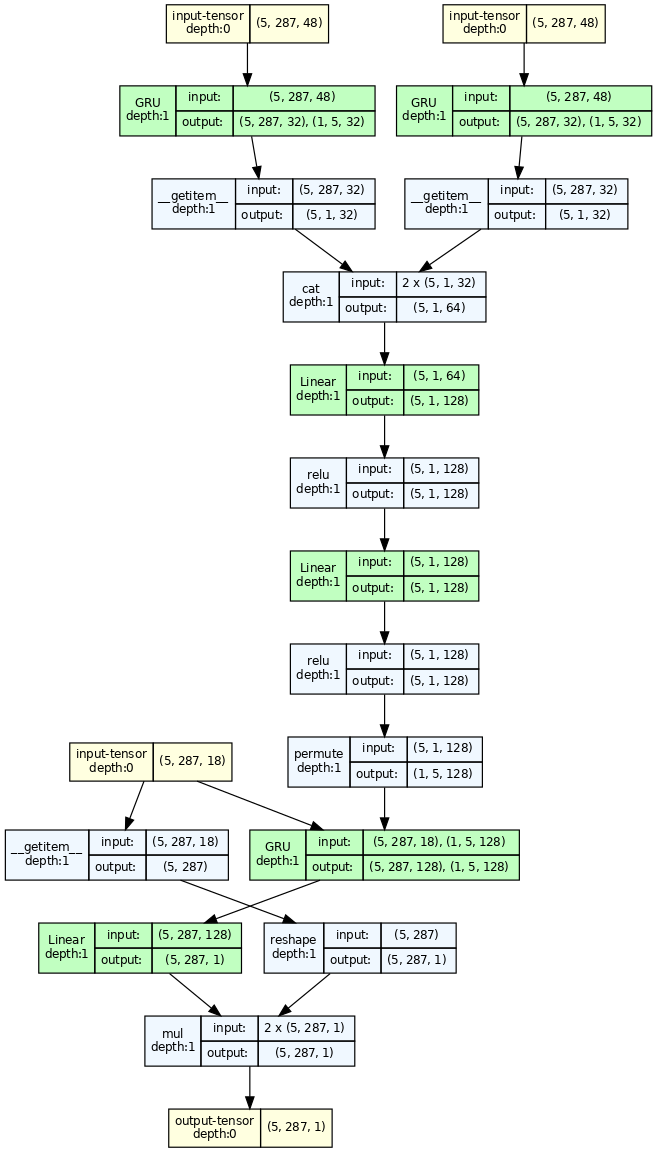
\includegraphics[height=.9\textheight]{chapters/3_models/imgs/grrun/grrunarchitecture.png}
	\caption{Recurren Neural Netowrk Based Model architecture visualization.}\label{fig:grrunarchitecture}
\end{figure}

\subsection{Training}
The model was trained to learn the trend of the instant energy production curve of the plant during gaps of variable lengths, ranging from a minimum of 60 timestamp to a maximum of 4 days, using variable dimensions for both \textit{before} and \textit{after}, ranging from 2 timestamps up to a maximum of 1 day.
These gaps were artificially generated in the training dataset and provided to the model
as described earlier, with attention to grouping gaps of the same length in
batches to avoid complications during training.

In this case, an \textit{Early Stopping}\cite{es} and \textit{Save Best} procedure were implemented
as well to ensure that the model always saves the best-performing model and to prevent
resource waste.

The validation dataset was applied in this phase to conduct an initial
and preliminary evaluation of the training process and highlight potential issues.
A normalization procedure was also applied to scale the prediction area with respect
to the ground truth area.
This allows the model to learn the shape of the curve and not exceed the limits
of energy production during the gap.

The Adam\cite{adam} optimizer was used, and the L1Loss\cite{loss} was applied as the loss function.
The batch size was set to 10, the learning rate ($\lambda$) was set to 0.0001,
a maximum of 100 epochs was set, and the patience was set to 20.

%Il modello è stato allenato per cercare di apprendere l'andamento della
%curva dell'energia istantanea prodotta dall'impianto durante buchi di 
%dimensione variabile che vanno da un minimo di 1 giorno ad un massimo di 4 giorni. Questi buchi sono stati generati artificialmente nel dataset di training e passati al modello come descritto in precedenza
%facendo attenzione a raggruppare in batch sempre buchi della stessa 
%dimensione per evitare complicazioni durante l'addestramento.
%Anche qui è stata implementata una procedura di \textit{Early Stopping} e \textit{Save Best}
%per garantire sempre di salvare il modello con le prestazioni migliori
%ed evitare spreco di risorse.
%Il dataset di validation è stato applicato in questa fase per poter
%effettuare una prima e sommaria valutazione della procedua di addestramento ed evidenziare potenziali problemi.
%Anche in questo caso è stata applicata una procedura di normalizzazione 
%dell'area della predizione rispetto a quella della ground thorught per
%far si che il modello apprenda a predirre la forma della curva e che non
%superi i limiti di energia prodotta durante il buco.
%L'ottimizzatore Adam è stato impiegato ed è stata applicata la L1Loss come loss function.
%Abbiamo impostato a 10 la batch size, a 0.01 il learning rate $\lambda$, un
%massimo di 100 epoche ed una patience pari a 20.

\begin{table}[H]
	\begin{center}
		\begin{tabular}[c]{l|l}
			\textbf{Total Parameters (\#)}     & 92737 \\
			\textbf{Trainable Parameters (\#)} & 92737 \\
			\textbf{Training Duration (s)}     & 49.0  \\
			\textbf{Model Size (KB)}           & 366.6
		\end{tabular}
	\end{center}
	\caption{RNN based model specification.}\label{tab:grrunspecs}
\end{table}

\begin{figure}[H]
	\centering
	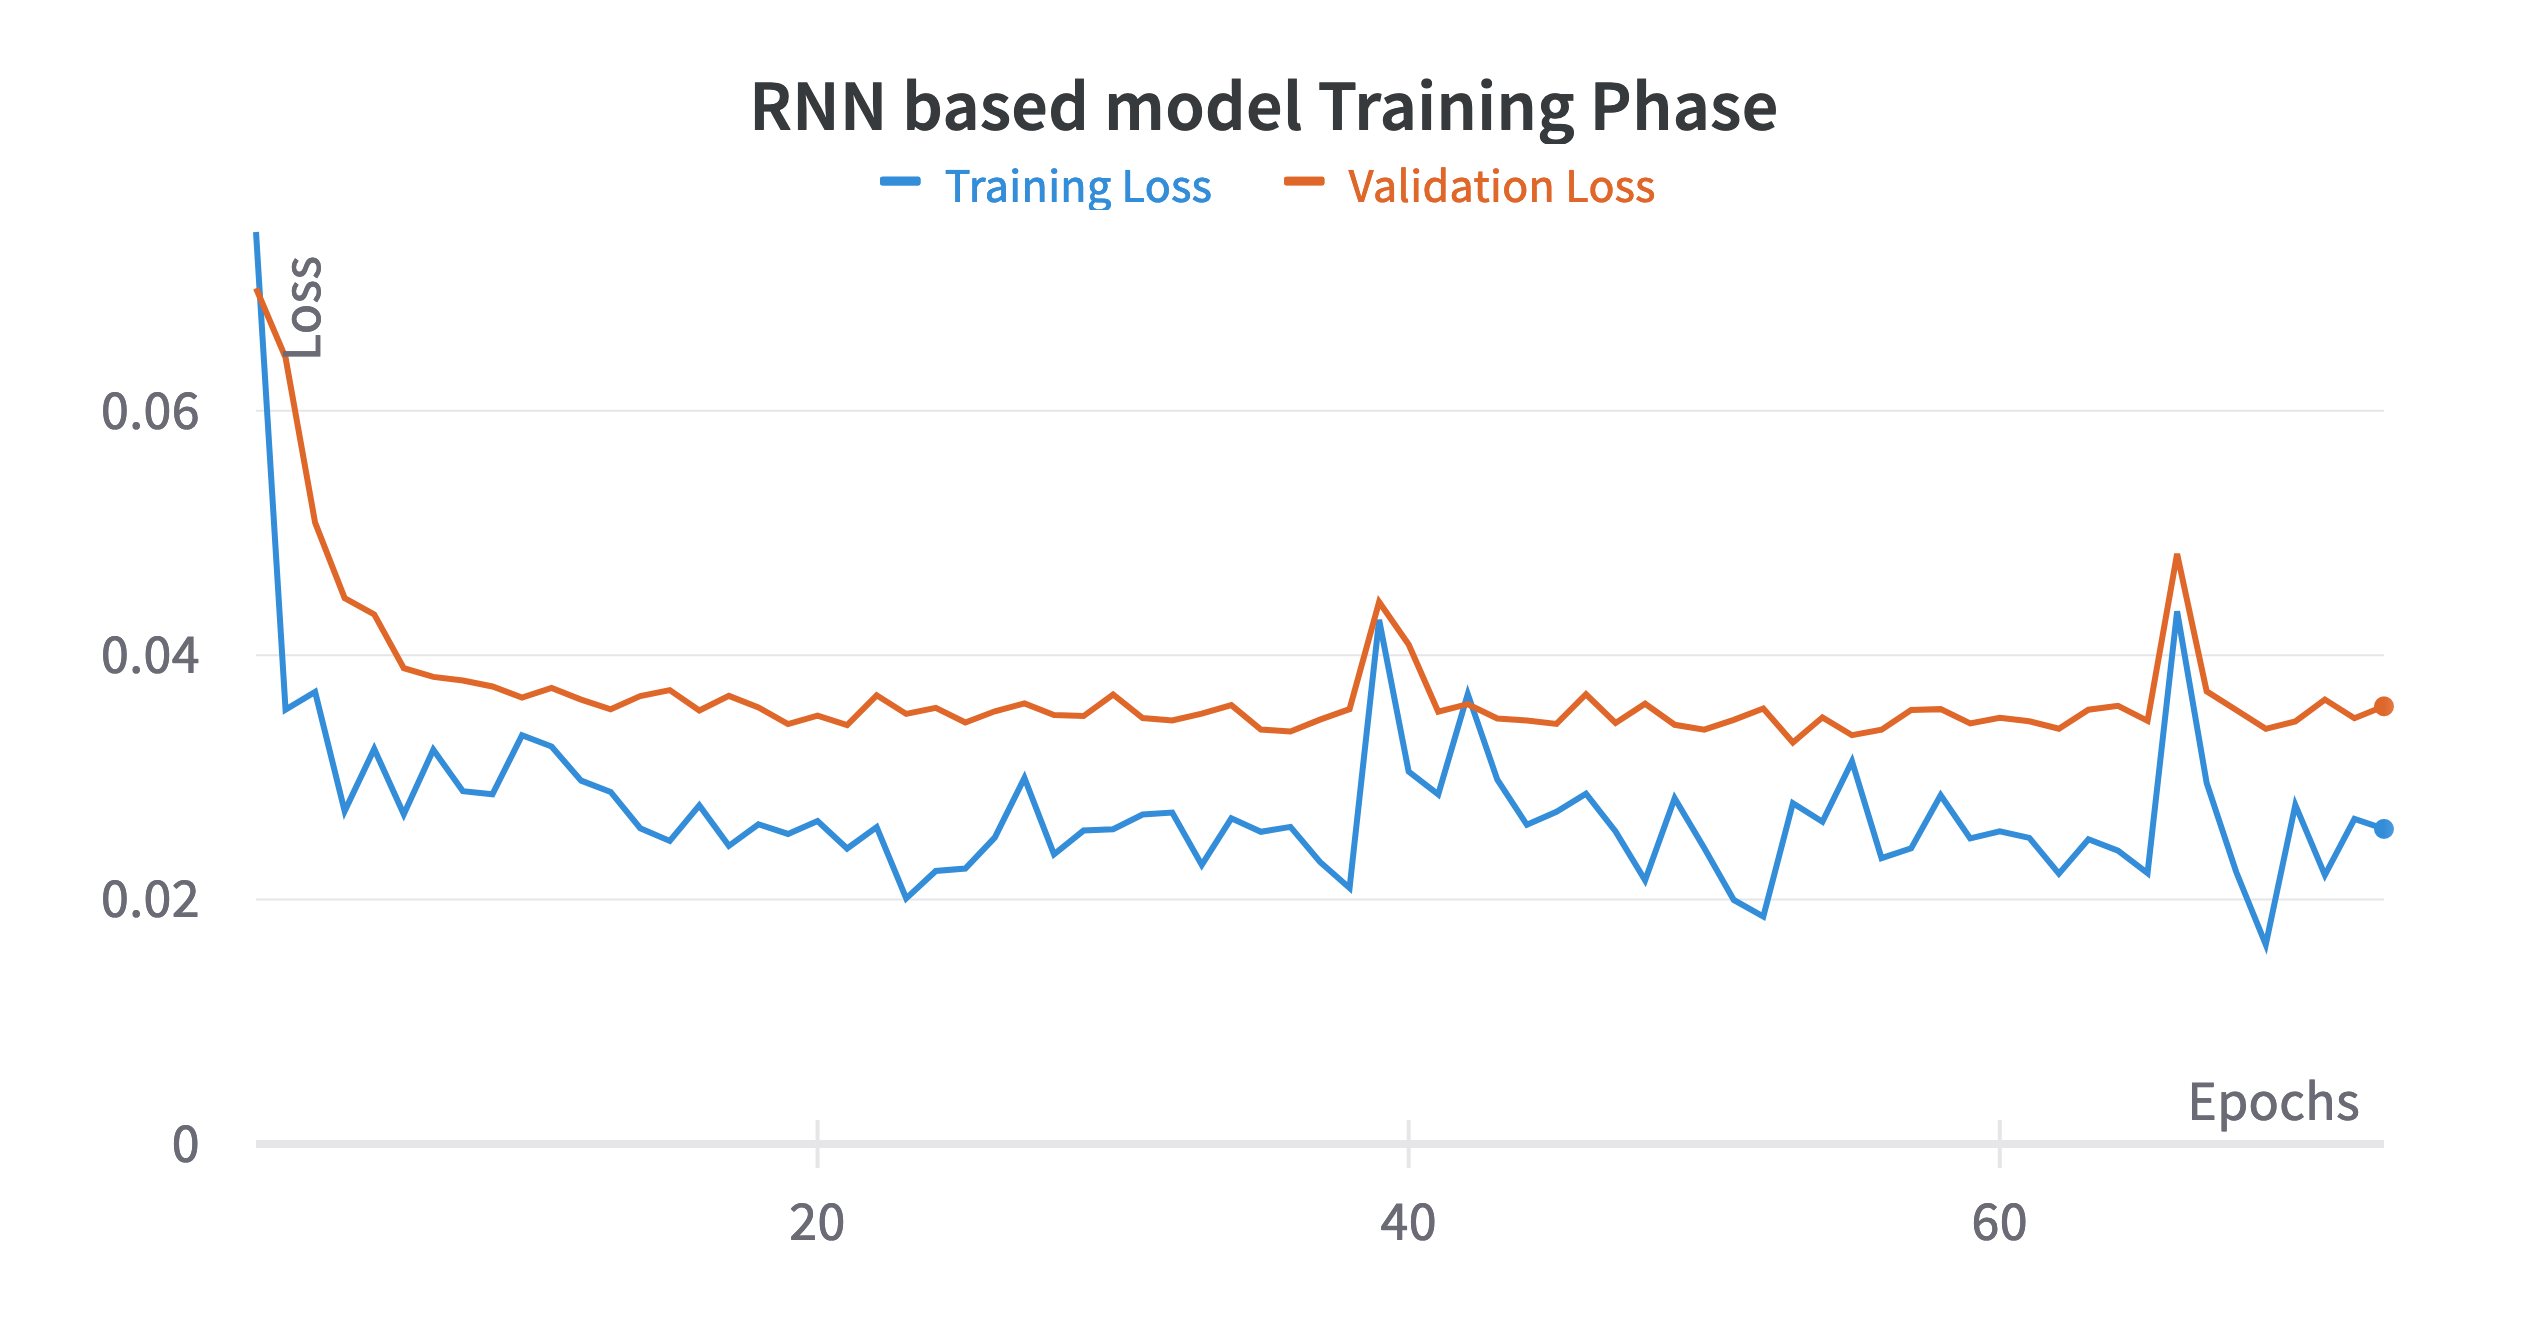
\includegraphics[width=.8\linewidth]{chapters/3_models/imgs/grrun/grruntraining.png}
	\caption{The chart displays the loss progression during the training phase.The blue line represents the Training Loss, while the orange line represents the Validation Loss.}
	\label{fig:grruntraining}
\end{figure}

\begin{figure}[H]
	\centering
	\begin{subfigure}{0.43\textwidth}
		\centering
		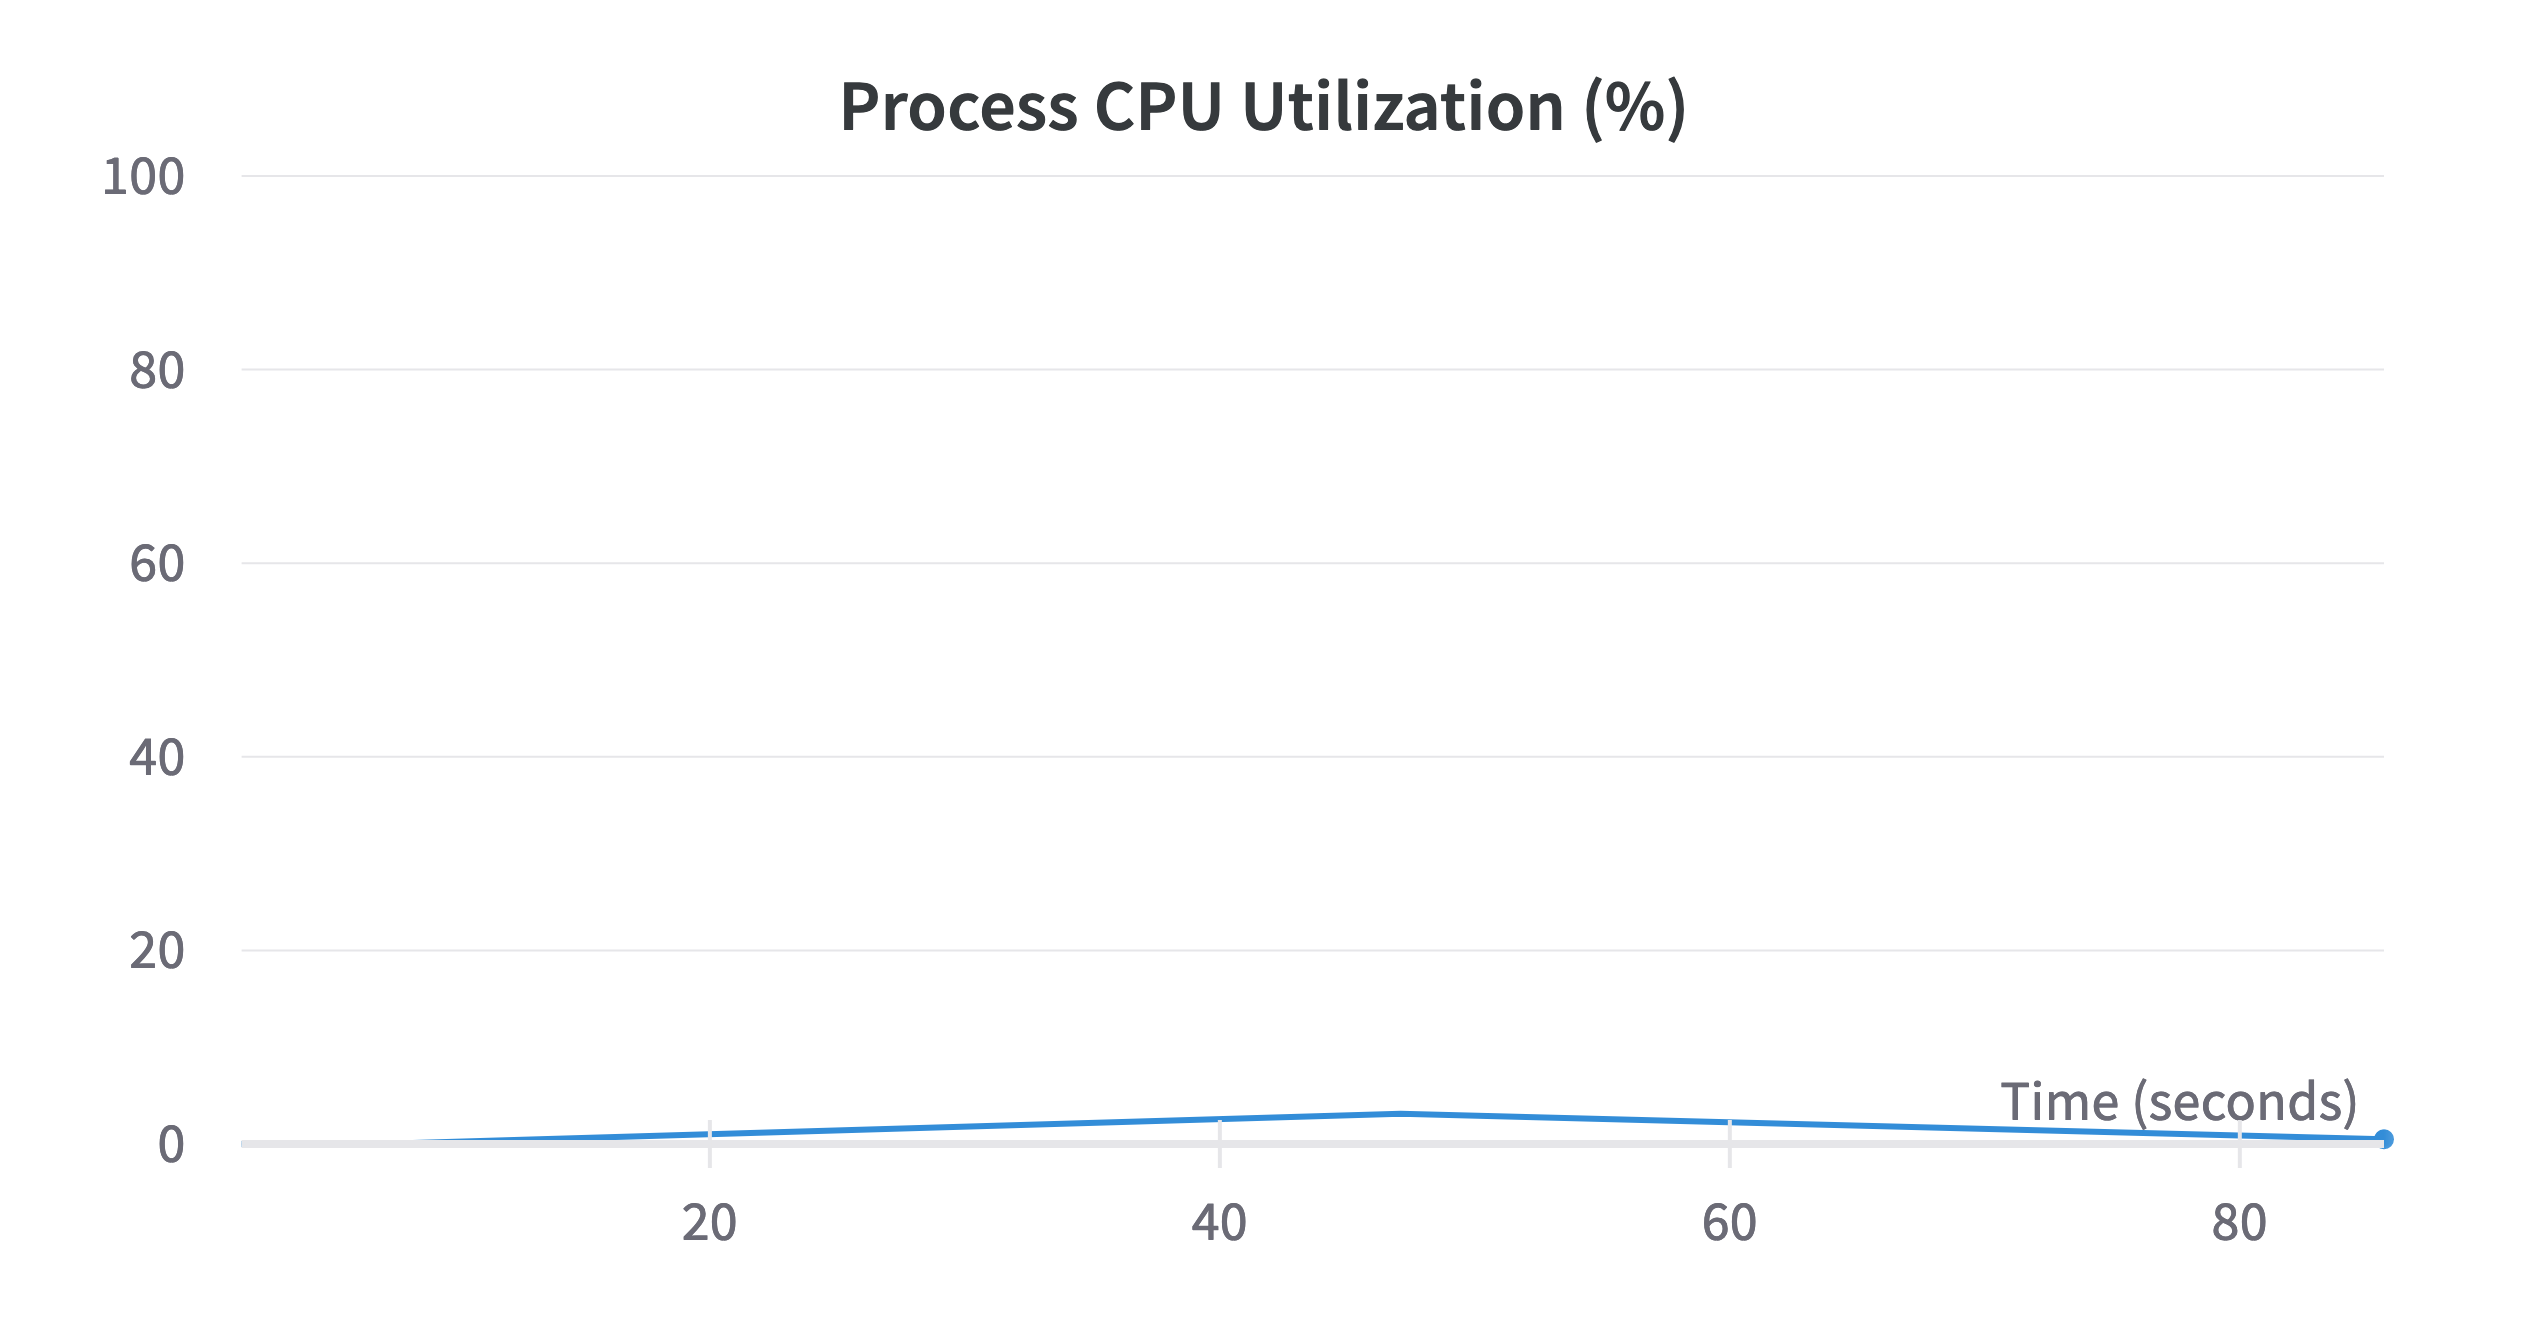
\includegraphics[width=\textwidth]{chapters/3_models/imgs/grrun/grruncputiliziation.png}
	\end{subfigure}
	\begin{subfigure}{0.43\textwidth}
		\centering
		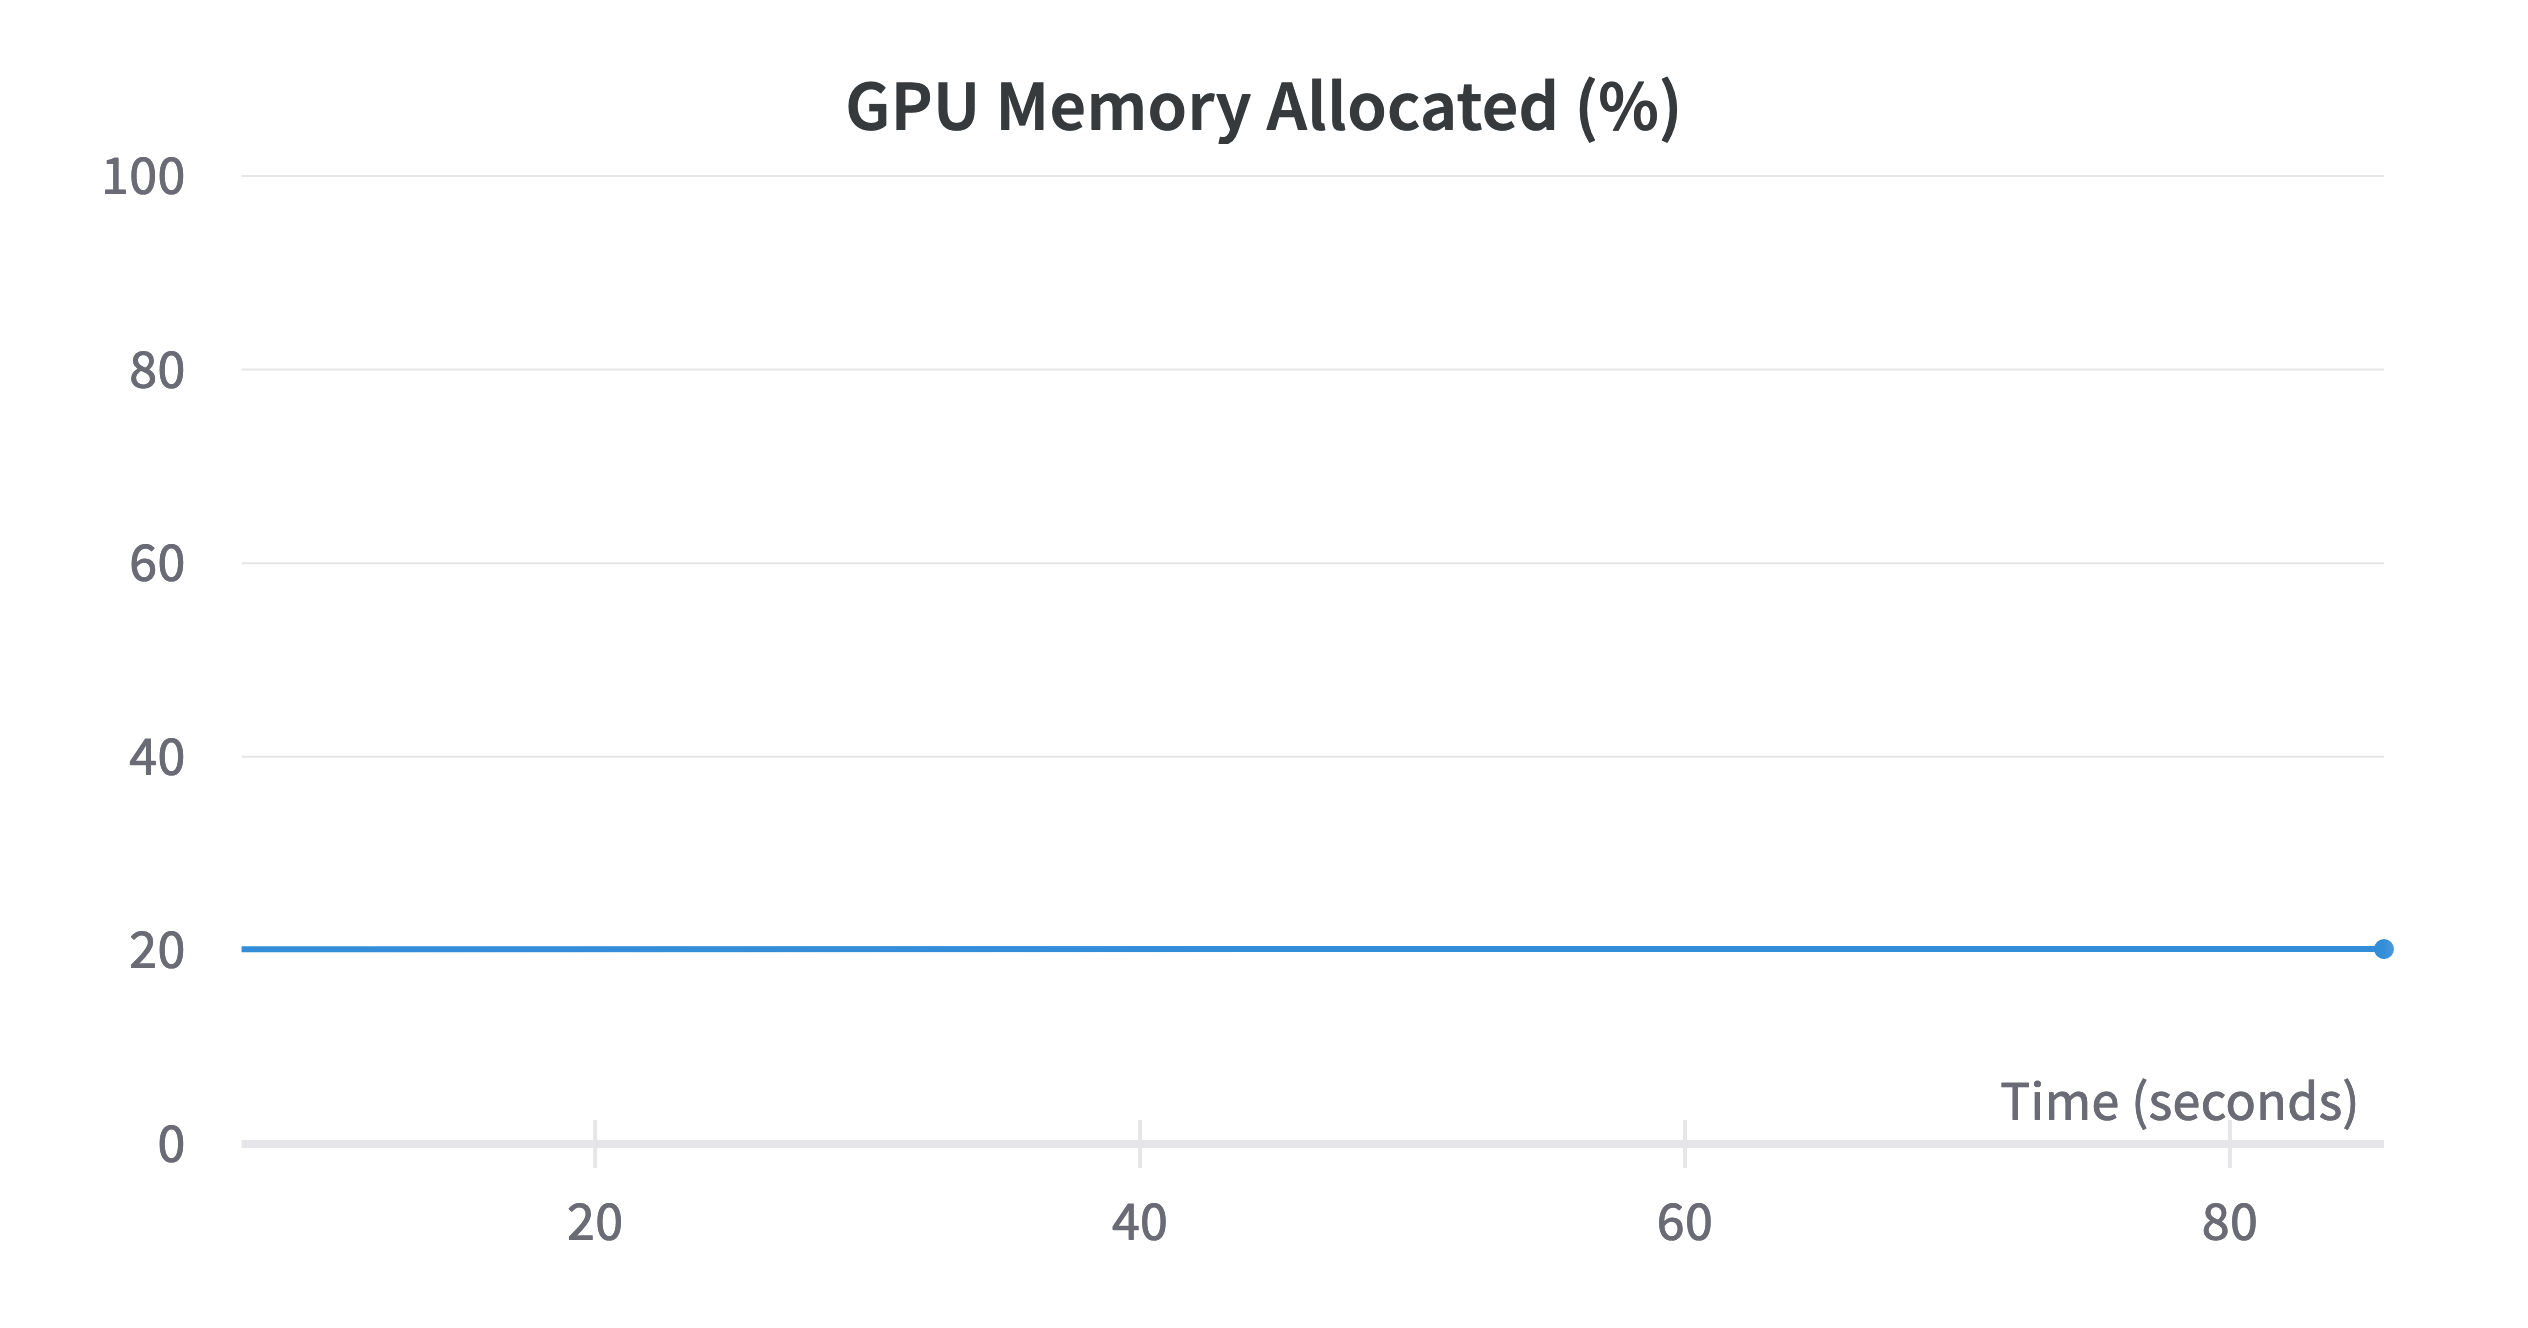
\includegraphics[width=\textwidth]{chapters/3_models/imgs/grrun/grrungpumemalloc.png}
	\end{subfigure}\\
	\begin{subfigure}{0.43\textwidth}
		\centering
		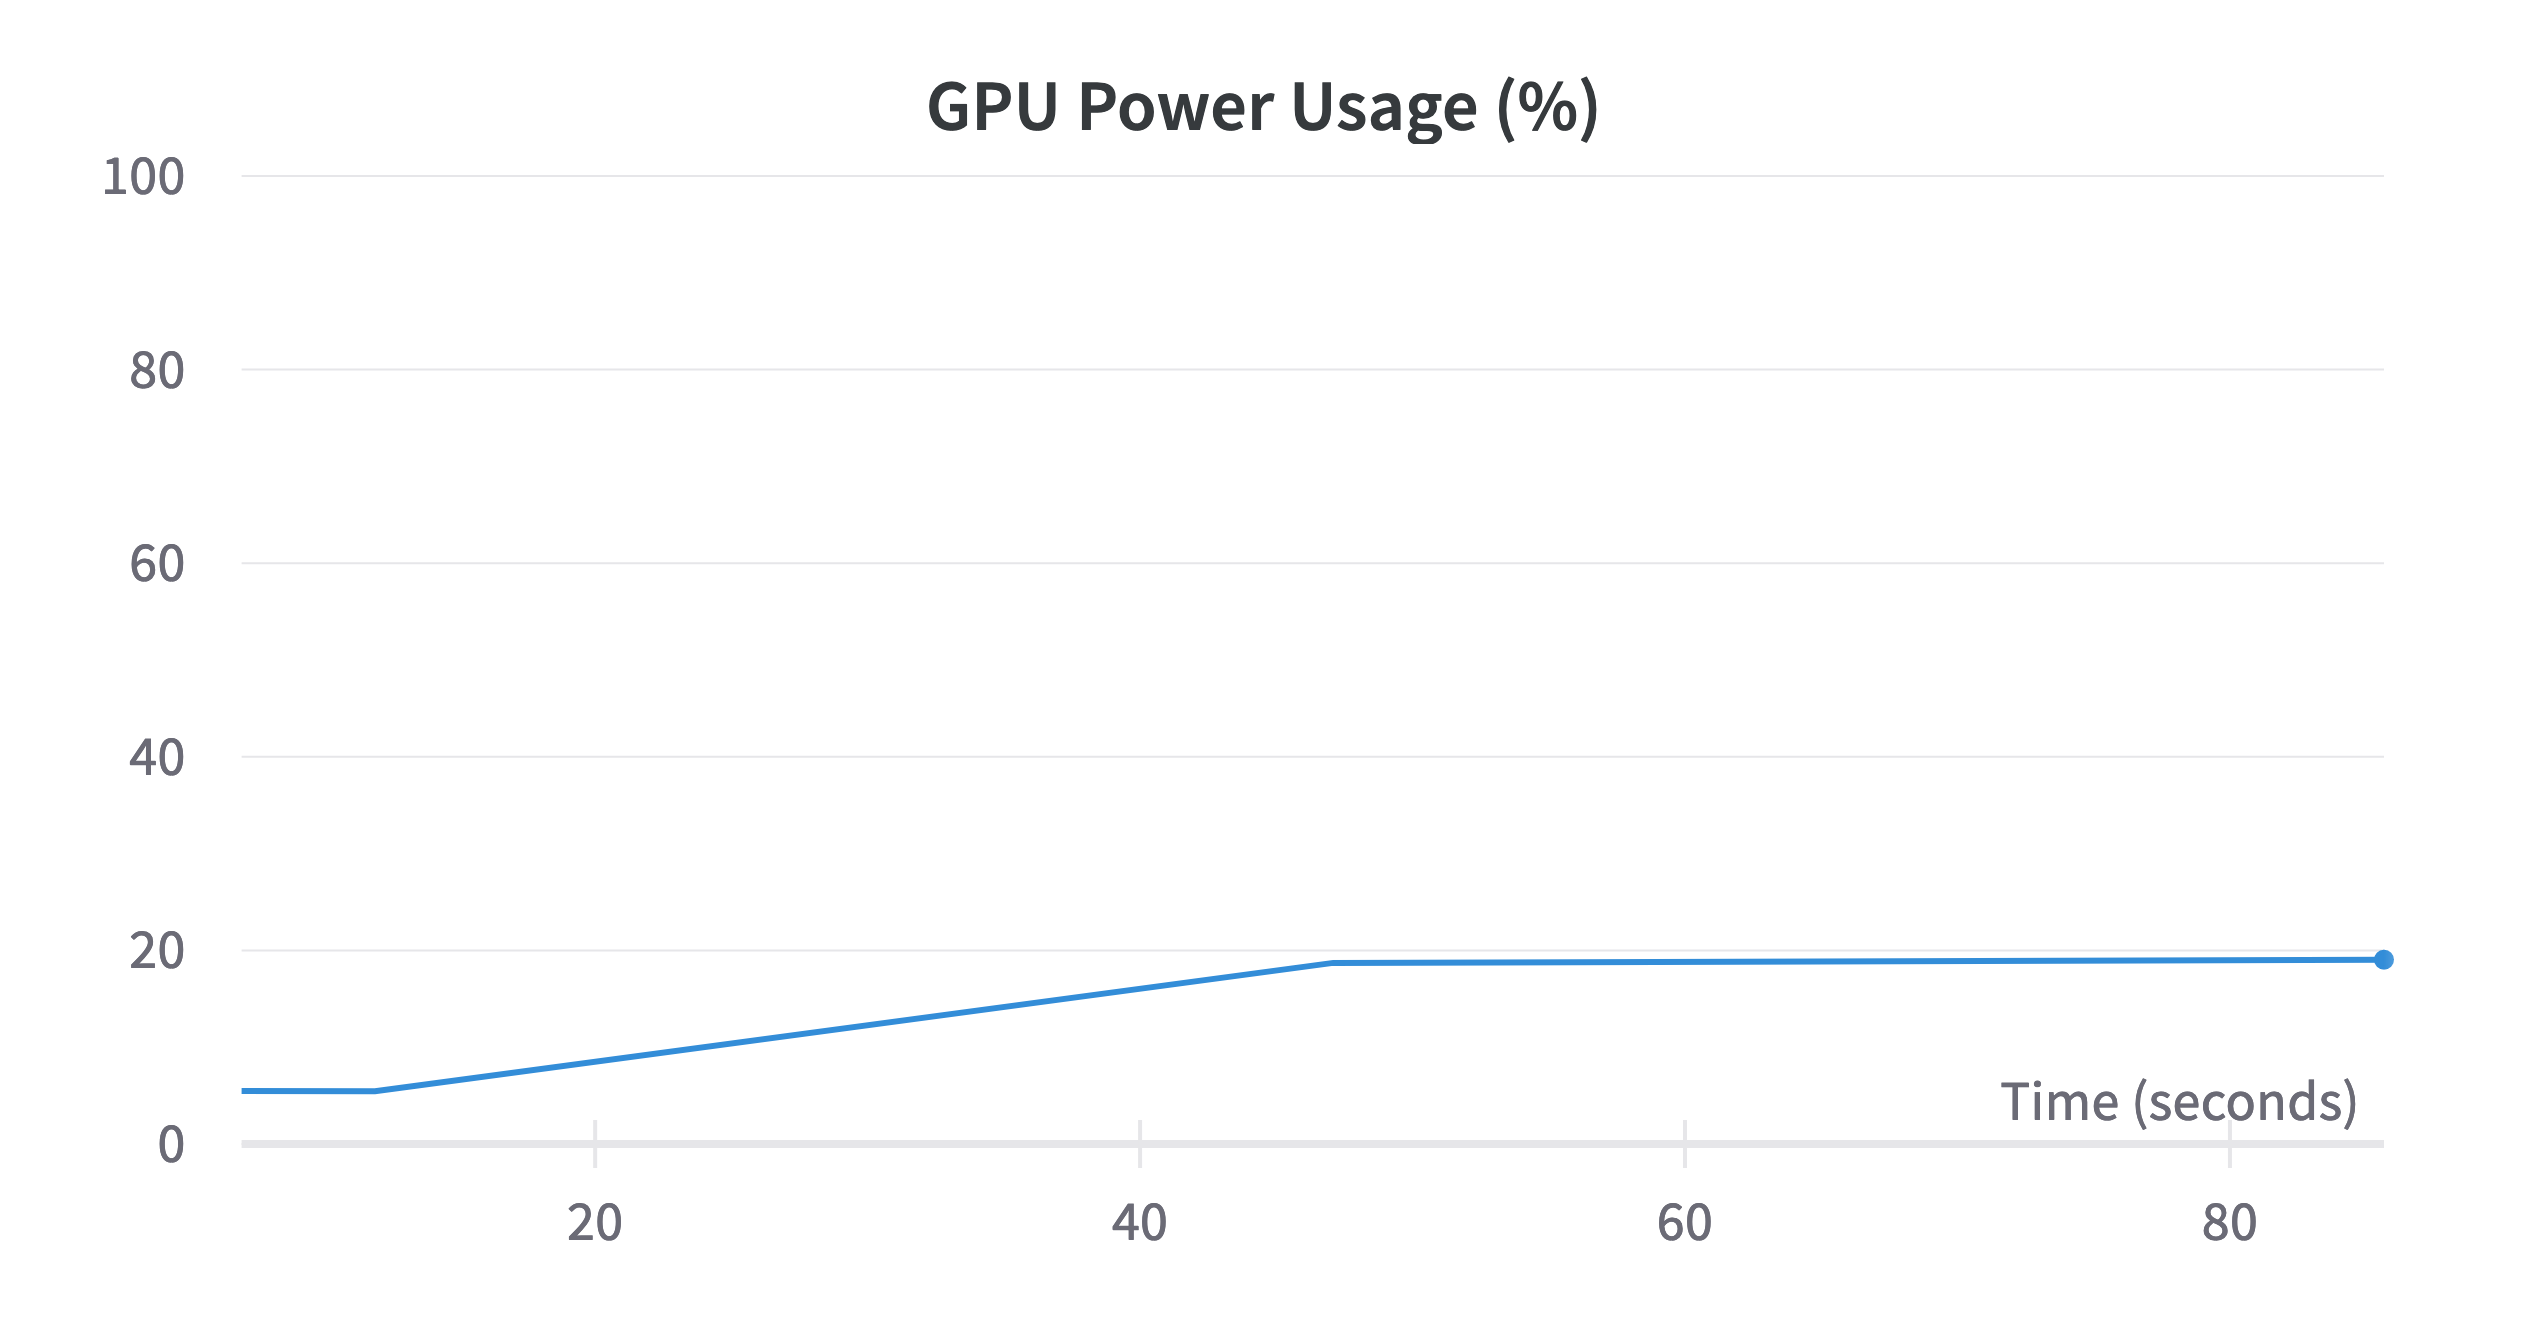
\includegraphics[width=\textwidth]{chapters/3_models/imgs/grrun/grrungpupowerusageperc.png}
	\end{subfigure}
	\begin{subfigure}{0.43\textwidth}
		\centering
		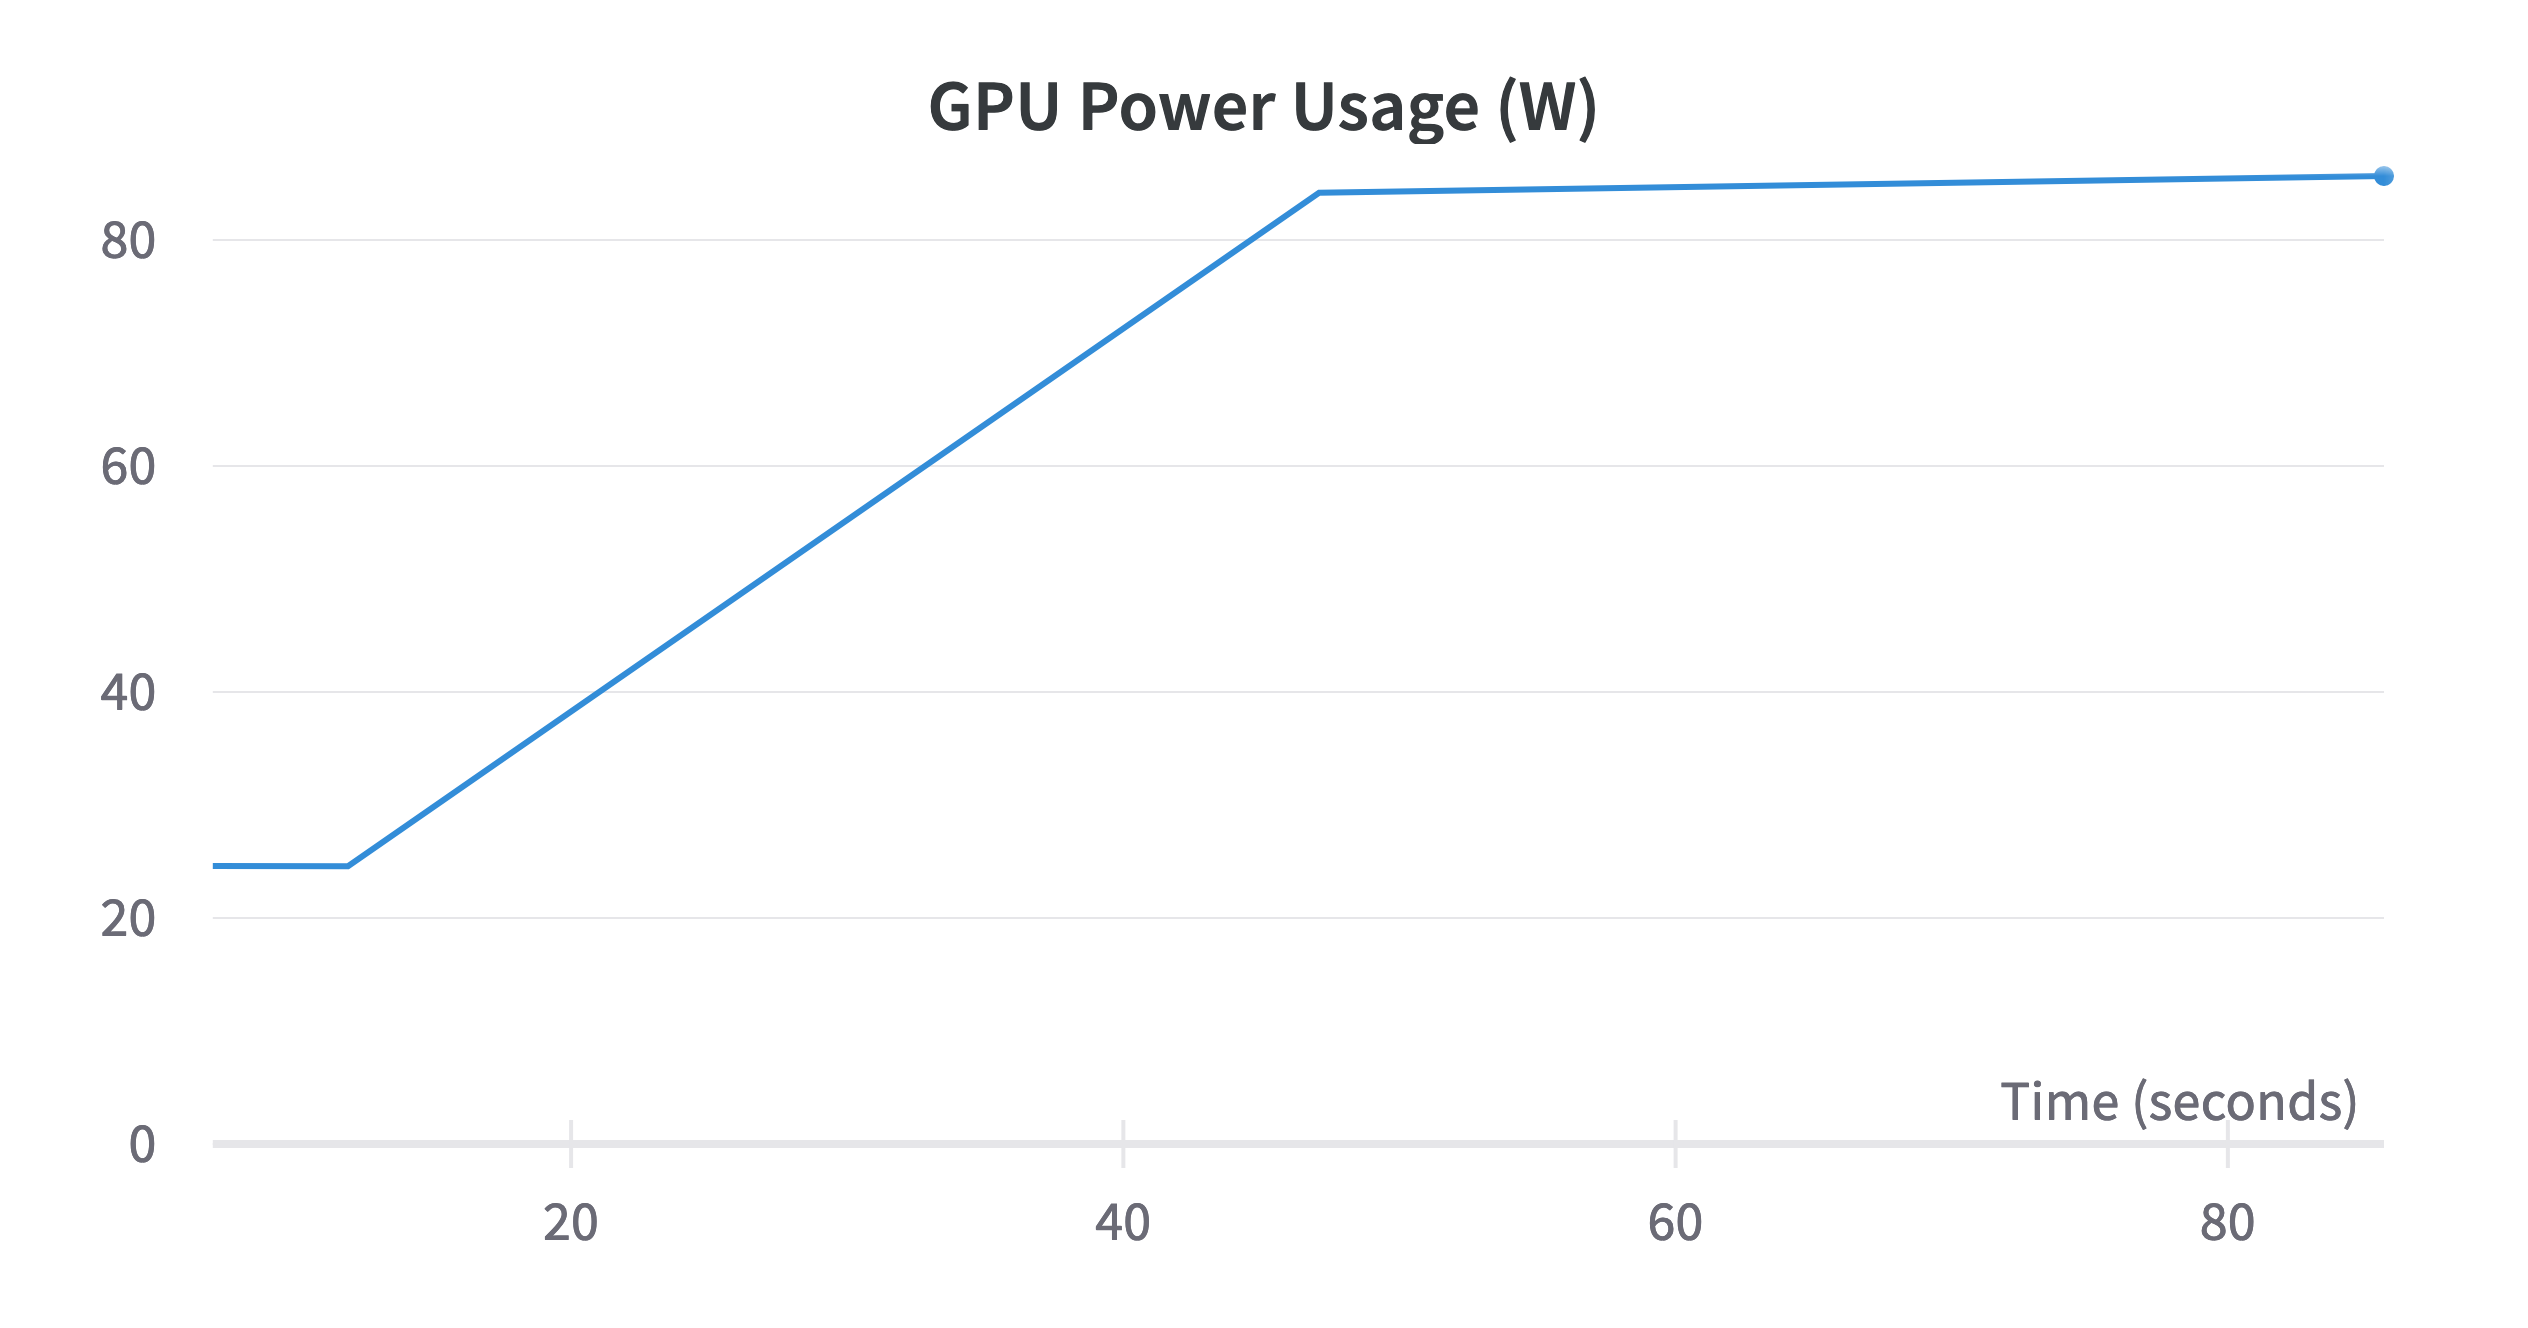
\includegraphics[width=\textwidth]{chapters/3_models/imgs/grrun/grrungpupowerw.png}
	\end{subfigure}\\
	\begin{subfigure}{0.43\textwidth}
		\centering
		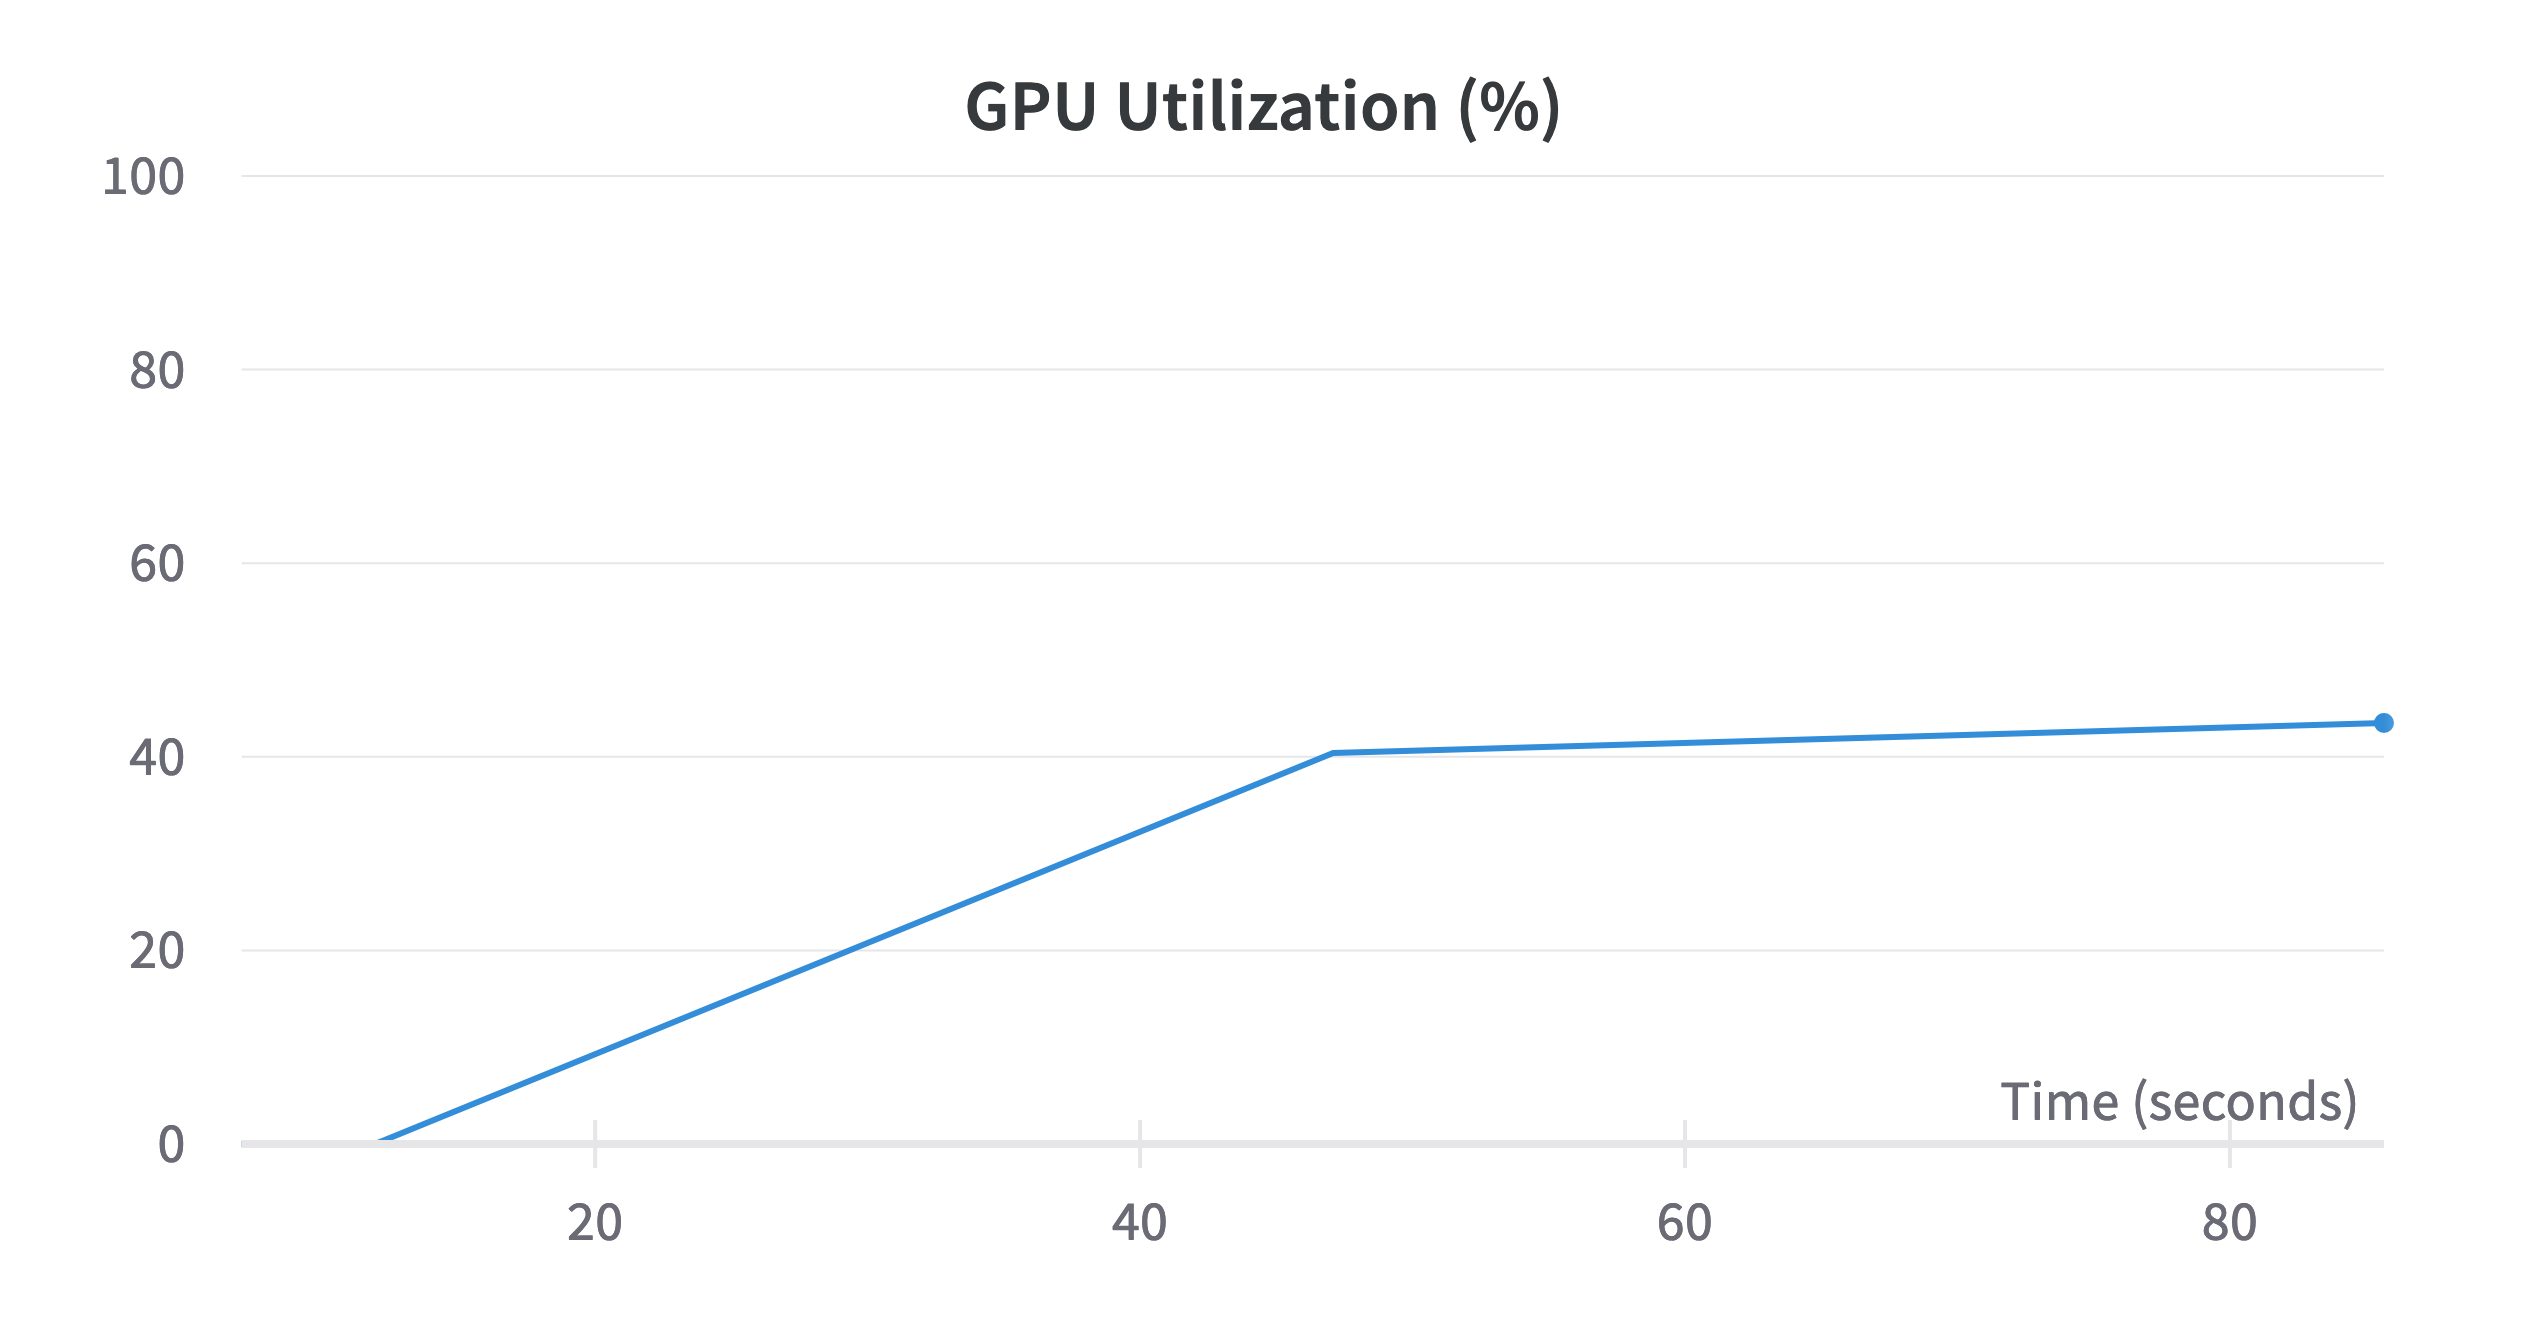
\includegraphics[width=\textwidth]{chapters/3_models/imgs/grrun/grrungputuilizationperc.png}
	\end{subfigure}
	\begin{subfigure}{0.43\textwidth}
		\centering
		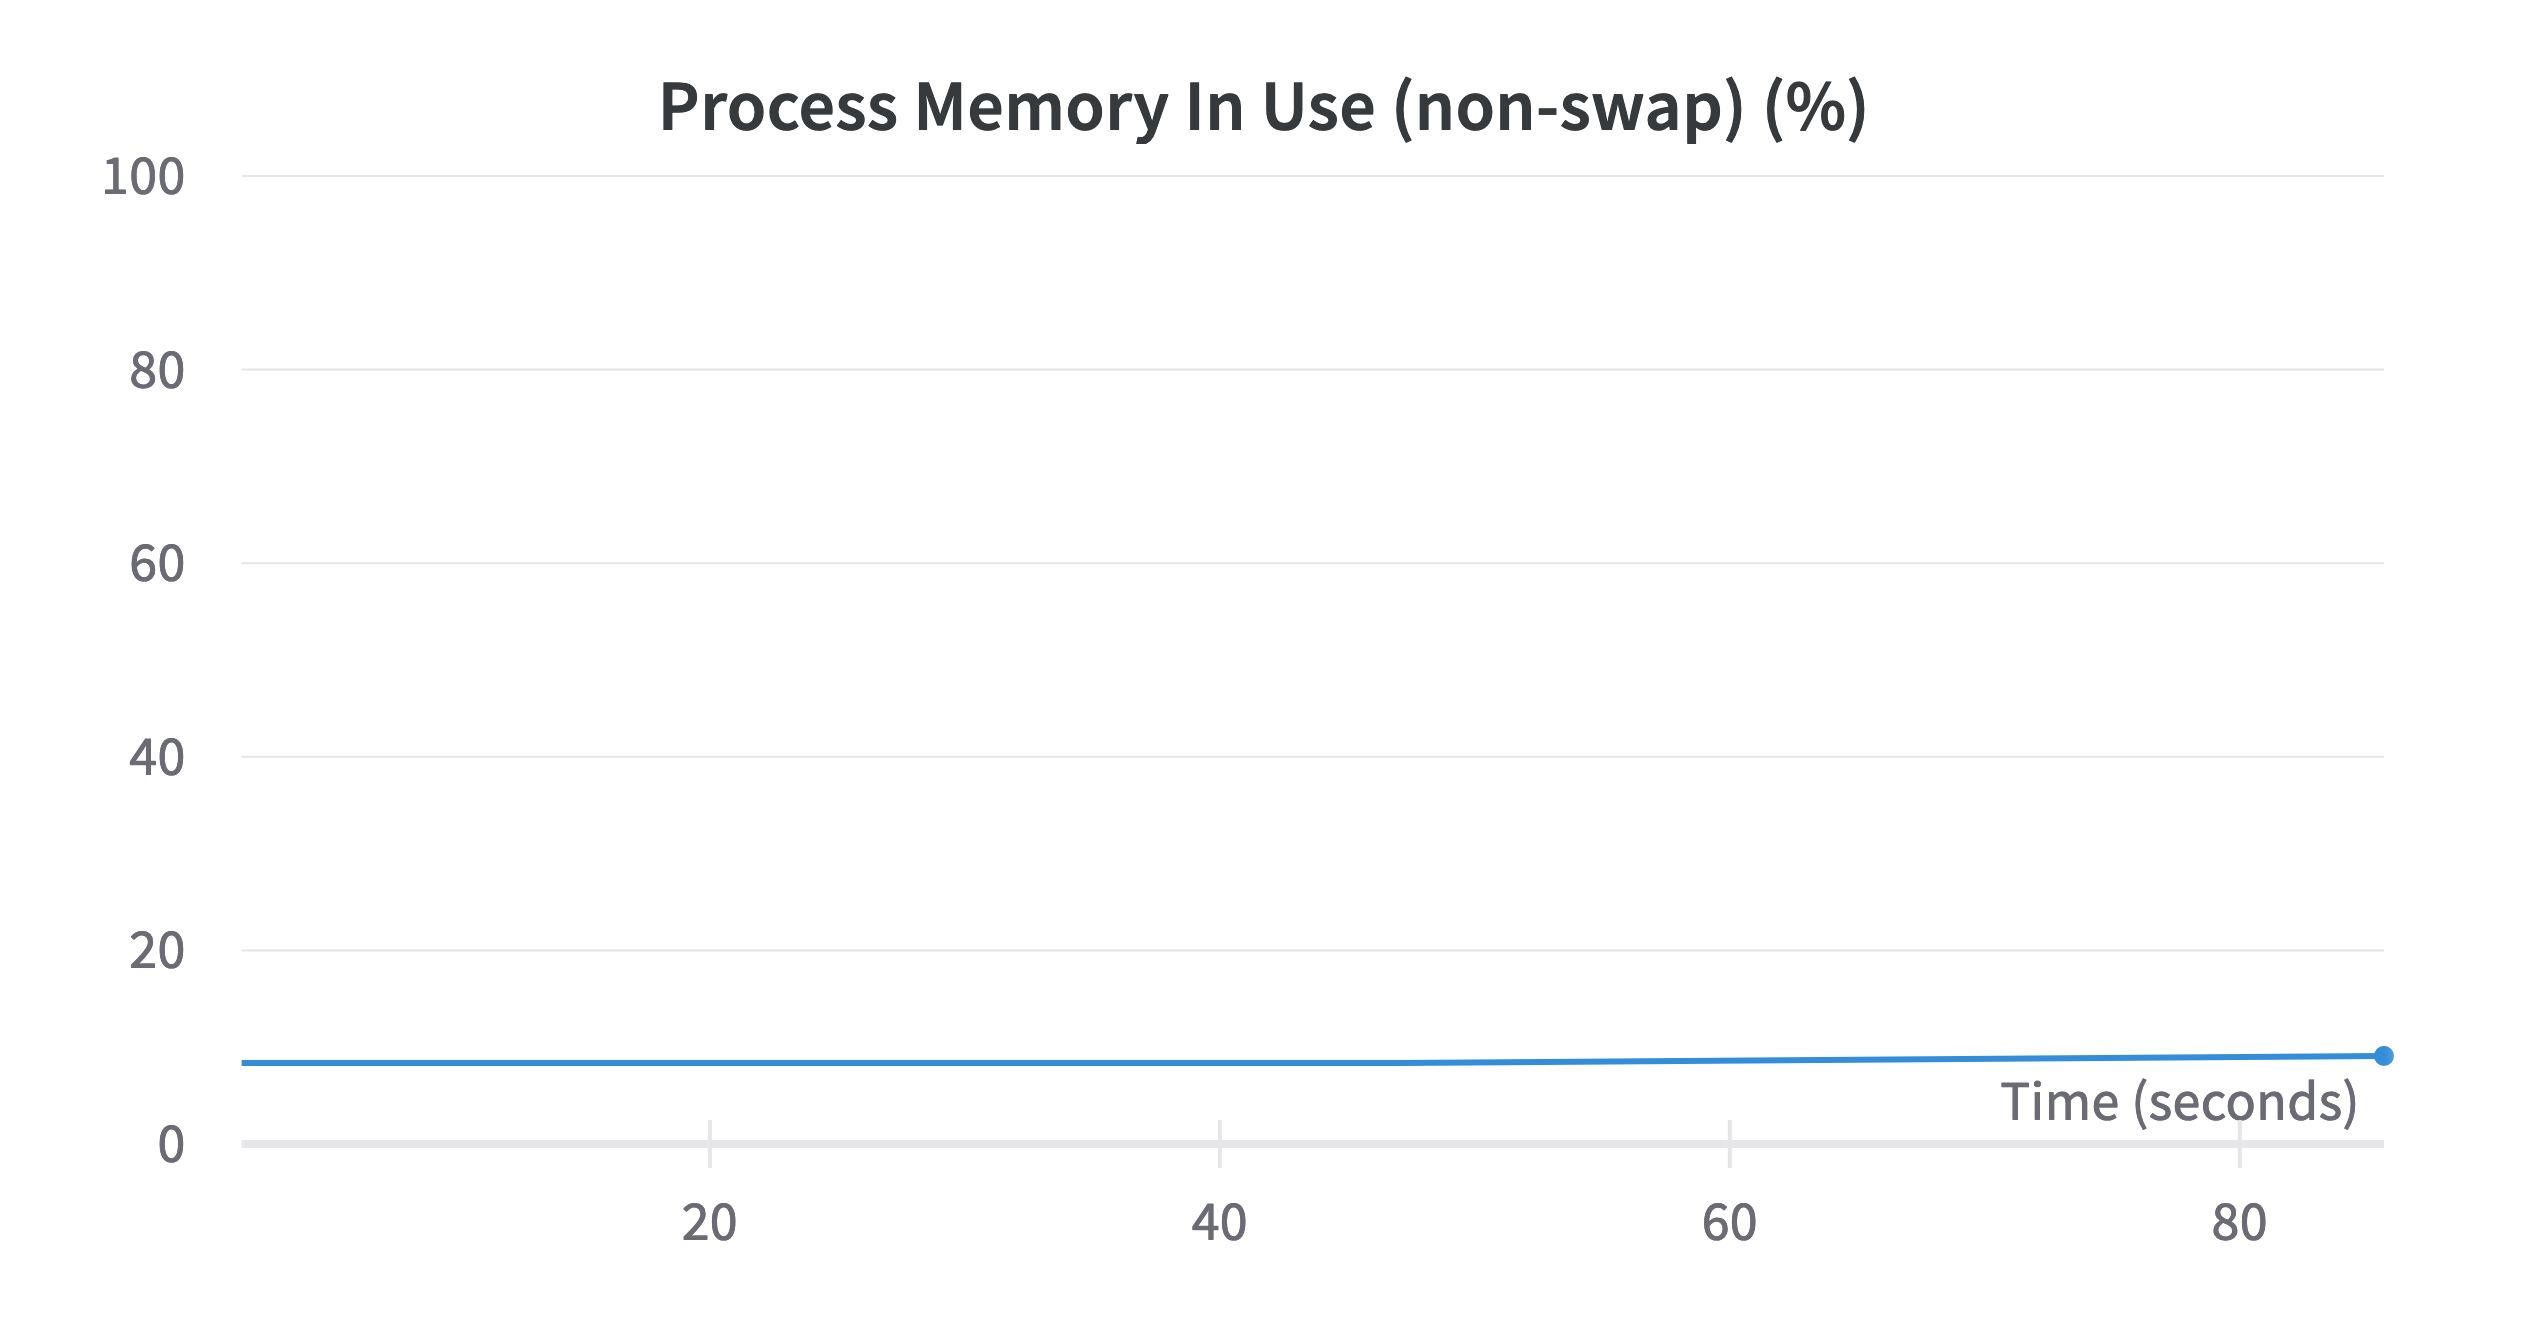
\includegraphics[width=\textwidth]{chapters/3_models/imgs/grrun/grrunmemusage.png}
	\end{subfigure}\\
	\caption{System resources utilized during the Training phase.}
	\label{fig:grrunsysusage}
\end{figure}


\begin{algorithm}[H]
	\caption{RNN model Training Algorithm}\label{alg:grruntraining}
	\begin{algorithmic}
		\Require train/validation datasets; Baseline Neural Network Model

		\State Batch Size $\gets$ 10
		\State Learning Rate $\lambda \gets$ 0.01
		\State Epochs $\gets$ 100
		\State Patience $\gets$ 20
		\State loss $\gets$ L1Loss()
		\State Optimizer $\gets$ Adam Optimizer
		\State Min Gap size $\gets$ 1 day
		\State Max Gap size $\gets$ 4 days
		\State
		\For{\textbf{each} epoch \textbf{in} epochs}
		\For{\textbf{each} (batch\_id, before, after, future, target) \textbf{in} train.next\_batch()}

		\State train\_prediction $\gets$ model(before, after, future) \Comment{Model inference}
		\State train\_prediction $\gets \frac{\text{train\_prediction} \cdot \sum\text{train\_prediction}}{\sum target}$ \Comment{Area normalization}
		\State train\_loss $\gets$ loss(train\_prediction, target)
		\State Optimizer step
		\State Back Propagation
		\EndFor
		\State stop computing gradient
		\For{\textbf{each} (batch\_id, vb, va, vf, vt) \textbf{in} validation.next\_batch()}
		\State val\_prediction $\gets$ model(vb, va, vf) \Comment{Model inference}
		\State val\_prediction $\gets \frac{\text{val\_prediction} \cdot \sum\text{val\_prediction}}{\sum vt}$ \Comment{Area normalization}
		\State val\_loss $\gets$ loss(val\_prediction, vt)
		\EndFor

		\State check for Early Stopping
		\State check for Save Best Result
		\State start computing gradient
		\EndFor
	\end{algorithmic}
\end{algorithm}

